% ---------------------------------------------------------------------------
% Author guideline and sample document for EG publication using LaTeX2e input
% D.Fellner, v1.13, Nov 13, 2007

\documentclass{egpubl}
\usepackage{EGVMV16}

% --- for  Annual CONFERENCE
% \ConferenceSubmission % uncomment for Conference submission
% \ConferencePaper      % uncomment for (final) Conference Paper
% \STAR                 % uncomment for STAR contribution
% \Tutorial             % uncomment for Tutorial contribution
% \ShortPresentation    % uncomment for (final) Short Conference Presentation
%
% --- for  CGF Journal
% \JournalSubmission    % uncomment for submission to Computer Graphics Forum
% \JournalPaper         % uncomment for final version of Journal Paper
%
% --- for  CGF Journal: special issue
% \SpecialIssueSubmission    % uncomment for submission to Computer Graphics Forum, special issue
% \SpecialIssuePaper         % uncomment for final version of Journal Paper, special issue
%
% --- for  EG Workshop Proceedings
 \WsSubmission    % uncomment for submission to EG Workshop
% \WsPaper         % uncomment for final version of EG Workshop contribution
%
\electronicVersion % can be used both for the printed and electronic version

% !! *please* don't change anything above
% !! unless you REALLY know what you are doing
% ------------------------------------------------------------------------

% for including postscript figures
% mind: package option 'draft' will replace PS figure by a filname within a frame
\ifpdf \usepackage[pdftex]{graphicx} \pdfcompresslevel=9
\else \usepackage[dvips]{graphicx} \fi

\PrintedOrElectronic

% prepare for electronic version of your document
\usepackage{t1enc,dfadobe}

\usepackage{egweblnk}
\usepackage{cite}
\usepackage{amsmath}
\usepackage{amssymb}

% For backwards compatibility to old LaTeX type font selection.
% Uncomment if your document adheres to LaTeX2e recommendations.
% \let\rm=\rmfamily    \let\sf=\sffamily    \let\tt=\ttfamily
% \let\it=\itshape     \let\sl=\slshape     \let\sc=\scshape
% \let\bf=\bfseries

% end of prologue

\DeclareMathOperator*{\argmin}{argmin}   

% !TEX root = EGauthorGuidelines-VMV16-fin.tex
% ---------------------------------------------------------------------
% EG author guidelines plus sample file for EG publication using LaTeX2e input
% D.Fellner, v1.17, Sep 23, 2010

  
\usepackage{amsmath}
\usepackage{amsfonts}

\title[3D Face Reconstruction with Silhouette Constraints]%
      {3D Face Reconstruction with Silhouette Constraints}

% for anonymous conference submission please enter your SUBMISSION ID
% instead of the author's name (and leave the affiliation blank) !!
\author[Q. Hu \& M. Zwicker \& P. Favaro]
       {Q. Hu \, M. Zwicker
        and P. Favaro
        \\
% For Computer Graphics Forum: Please use the abbreviation of your first name.
         Institute of Computer Science, University of Bern, Switzerland\\
%         $^2$Institut f{\"u}r ComputerGraphik \& Wissensvisualisierung, TU Graz, Austria
%        $^2$ Another Department to illustrate the use in papers from authors
%             with different affiliations
       }
        
% For Computer Graphics Forum: Please use the abbreviation of your first name.
         %$^1$TU Darmstadt \& Fraunhofer IGD, Germany\\
%         $^2$Institut f{\"u}r ComputerGraphik \& Wissensvisualisierung, TU Graz, Austria
%        $^2$ Another Department to illustrate the use in papers from authors
%             with different affiliations
%       }
% ------------------------------------------------------------------------

% if the Editors-in-Chief have given you the data, you may uncomment
% the following five lines and insert it here
%
% \volume{27}   % the volume in which the issue will be published;
% \issue{1}     % the issue number of the publication
% \pStartPage{1}      % set starting page
\usepackage{graphicx,booktabs,multirow}


%-------------------------------------------------------------------------
\begin{document}



\teaser{
  %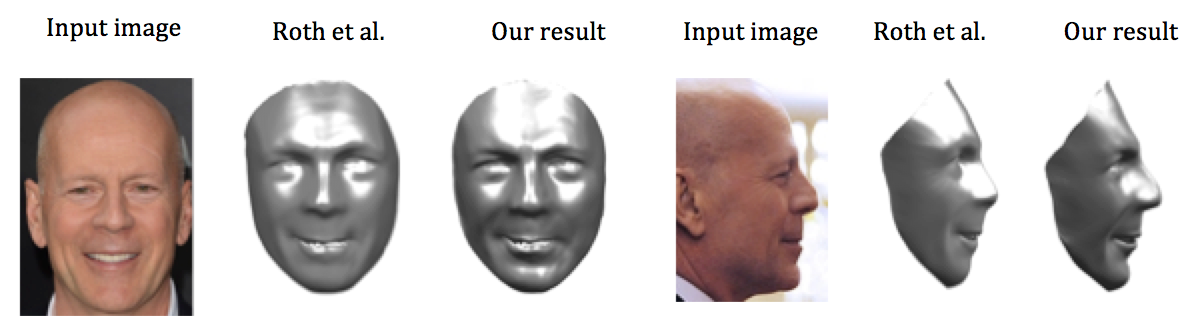
\includegraphics[width=\linewidth]{figures/teaser.png}
   
\includegraphics[height=.21\linewidth, width=.15\linewidth,trim=0  -20 0 0]{figures/teaser/bw_front.jpg}  
  \includegraphics[height=.21\linewidth,width=.15\linewidth,trim=130  -40 90 0,clip]{figures/teaser/roth_bw_front.eps}  
  \includegraphics[height=.21\linewidth,width=.15\linewidth,trim=130  -40 90 0,clip]{figures/teaser/roth_bw_front.eps}    
  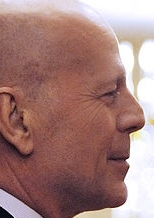
\includegraphics[height=.21\linewidth,width=.15\linewidth,trim=0  -20 0 0]{figures/teaser/bw_profile.jpg}
  \includegraphics[height=.21\linewidth,width=.15\linewidth,trim=130  -40 110 0,clip]{figures/teaser/roth_bw_profile.eps}  
  \includegraphics[height=.21\linewidth,width=.15\linewidth,trim=130  -40 90 0,clip]{figures/teaser/bw_profile.eps}      
  \centering
   \caption{We introduce silhouette constraints to improve the quality of unconstrained 3D face reconstruction. Here, we show a comparison between the state of the art approach by Roth et al. \cite{Roth:2015:UFR} and our technique. The 2nd and 5th column are the results from ~\cite{Roth:2015:UFR}, the 3rd and 6th column are our results. Note how our approach follows more faithfully the silhouettes of the input images, especially around the nose region.}
 \label{fig:teaser}
}

\maketitle

\begin{abstract}
In this paper we introduce silhouette constraints to improve the quality of unconstrained 3D face reconstruction. Previously, state of the art unconstrained 3D face reconstruction techniques relied solely on photometric consistency and matching sparse facial landmarks. We show that constraining the silhouettes of the 3D reconstruction to match silhouettes in the input images can further improve reconstruction quality. Our technique automatically detects silhouettes and iteratively matches silhouette points computed from the current 3D reconstruction with silhouettes in the input images. We demonstrate that our results improve on the previous state of the art in unconstrained 3D face reconstruction and that our additional constraints can easily be included in the iterative reconstruction at little additional cost.
%\begin{classification} % according to http://www.acm.org/class/1998/
%\CCScat{Computer Graphics}{I.3.3}{Picture/Image Generation}{Line and curve generation}
%\end{classification}

\end{abstract}


%-------------------------------------------------------------------------
\section{Introduction}

We consider the problem of 3D face reconstruction from internet photo collections. Our goal is to reconstruct 3D models of individuals from collections of images in uncontrolled environments, including variations in illumination, pose, and expression, which has been called ``face reconstruction in the wild'' \cite{Kemelmacher-Shlizerman:2011:FRW} or ``unconstrained 3D face reconstruction'' \cite{Roth:2015:UFR}. Such 3D reconstructions can be useful for face and expression recognition \cite{Liu:2005:PFR,Wang:2006:FER}, or to produce facial animations \cite{Li:2013:RFA}.

Our work is inspired by recent progress in unconstrained face recognition by Roth et al. \cite{Roth:2015:UFR}. They leverage state of the art photometric stereo techniques, recent advances in 2D facial landmark estimation, and a full 3D face representation (instead of 2.5D height fields) to obtain impressive results, considering that the input consists of images under various illumination conditions, with different poses and facial expressions, and neither video or stereo data is included in the input. Nonetheless, the quality of the 3D reconstructions is limited since the only constraints on the reconstruction are photometric consistency and correspondence with sparse facial landmarks. 

In this paper, we introduce silhouette constraints to improve the quality of unconstrained 3D face reconstruction. Our main idea is to extract silhouette points on the 3D reconstruction, and match them with automatically detected silhouette points in the input images. We include these constraints in the 3D reconstruction objective, which we solve in an iterative process. In each iteration step, we recompute the silhouette points using the current 3D reconstruction and update the corresponding contraints in the objective. As a consequence, the silhouettes of the 3D reconstruction converge towards the silhouettes in the input images. Our results demonstrate that the new silhouette constraints lead to higher reconstruction quality.

The rest of this paper is organized as follows: We first review related work in Section~\ref{sec:related}, and provide a brief overview of state of the art unconstrained face reconstruction as proposed by Roth et al.~\cite{Roth:2015:UFR} in Section~\ref{sec:unconstrainedfacereconstruction}. In Section~\ref{sec:silhouetteconstraints} we introduce the novel silhouette constraints as our main contribution. Finally, we present results in Section~\ref{sec:results} and conclude in Section~\ref{sec:conclusions}.


%-------------------------------------------------------------------------
\section{Related work}
\label{sec:related}

\paragraph*{Face Reconstruction from Image Collections.} Face reconstruction ``in the wild'' from collections of images under uncontrolled illumination, and with varying facial pose and expressions, has been a long standing problem in computer vision. State of the art methods are mostly based on photometric stereo, such as the pioneering work by Kemelmacher-Shlizerman and Seitz \cite{Kemelmacher-Shlizerman:2011:FRW}, and its extension to video input \cite{Suwajanakorn2014}. This approach has been improved recently by Roth et al.~\cite{Roth:2015:UFR} who solve for a full 3D mesh instead of a 2.5D height field, and leverage state of the art 2D facial landmark estimation \cite{Zan:2013:LCM}. We build on the work by Roth et al., but extend it to include silhouette constraints to overcome some of the limitations of photometric stereo.

\paragraph*{Face Tracking and Animation from Video.} Research in the Computer Graphics community has achieved impressive results for the problem of tracking, reconstructing, and animating faces based on video data. Generally, state of the art techniques represent faces and facial expressions using dynamic expression models, also called blendshape models \cite{Cao:2014:FWA}. While earlier work relied on RGBD video input \cite{Weise:2011:RPF,Li:2013:RFA,Bouaziz:2013:OMR}, it is now possible to solve the tracking and reconstruction problem based on RGB video data in real-time at impressive quality. \cite{Cao:2014:DDE,Cao:2015:RHF,GZCVVPT16,thies2016face}. The key idea in this work is to learn a regression model that maps 2D video frames to 3D facial landmarks, and then to register the DEM to the 3D landmarks \cite{Cao:2013:SRR}. While this approach required calibration for individual users, it has then been extended to a calibration-free approach that iteratively refines the model \cite{Cao:2014:DDE}. A most recent extension also synthesizes highly detailed geometry such as wrinkles \cite{Cao:2015:RHF}. The key difference to our work is that these techniques either require calibration for each user, or they rely on the coherence of video input to adapt the model in an iterative manner.


%-------------------------------------------------------------------------
\section{Unconstrained Face Reconstruction}
\label{sec:unconstrainedfacereconstruction}

Unconstrained 3D face reconstruction \cite{Roth:2015:UFR} takes as its input  a collection of facial photographs of an individual under uncrontrolled illumination and various poses and facial expresssions, and it returns a full 3D reconstruction of the individual's face represented by a mesh. The method proceeds by first detecting 2D landmarks on all input images using the approach by Yan et al. \cite{Yan:2013:LCM}. Next, a 3D template mesh is warped and projected to 2D to match the 2D landmarks. This leads to an initial, rough 3D reconstruction of the face, and a weak perspective projection matrix for each input image. Then they improve the 3D reconstruction by determining surface normals using a photometric stereo approach, and lastly they perform 3D reconstruction by refining the rough mesh to match the photometric normals. We briefly review the main components of this approach.

\paragraph*{Template Warping.} Given the 2D landmarks, denoted by a vector $W_i$, for all images $i$, and a template mesh with $p$ vertices, denoted by a $3p$ dimensional vector $X_0$, the goal is to find a warped mesh $X$ and weak projection matrices $P_i$, such that the landmarks on $X$ projected to 2D match the 2D landmarks $W_i$. The key idea is to use Laplacian surface editing \cite{Sorkine:2004:LSE} to perform mesh deformation. This leads to a minimization problem
%
\begin{align}
\label{eq:warptemplate}
E_{warp}(X,P_{i})=\|\mathcal{L}X - \mathcal{L}X_{0}\|^2+\lambda_{l}\sum_{i}{\|P_{i}D_{i}X-W_{i}\|^2},
\end{align} 
%
which expresses the intuition that the mesh Laplacian \cite{Meyer2003} $\mathcal{L}X$ of the deformed mesh should stay close to the mesh Laplacian of the template $\mathcal{L}X_{0}$. In addition, $D_{i}$ is a selection matrix picking out the landmarks that have a correspondence in image $i$, that is, it is a diagonal matrix with $1$ on the diagonal for the vertices corresponding to a landmark and $0$ everywhere else. 

Equation~\ref{eq:warptemplate} is solved iteratively. First, the projection matrices are obtained by fixing the template and solving for $P_i$, which is a linear least squares problem. Then, the $P_i$ are fixed and the deformed mesh $X$ is obtained in an iterative approach. This is necessary because the mesh Laplacians $\mathcal{L}X$ and $\mathcal{L}X_0$ are not rotation invariant. Hence, after each iteration step the mesh Laplacian $\mathcal{L}X_0$ of the template is rotated until it aligns with the Laplacian $\mathcal{L}X$ obtained in the previous step.

%First, in \cite{Roth15} they compute 2D landmarks for all images using the approach in [5]. With the 2D landmarks, Warp the 3D model on the images by project 3D landmarks on 2D landmarks on image. Estimate the weak prospecive projection matrix $P_{i}$ for each image. Deform the 3D template using laplacian surface editing and adapt for the lanmark constraints until convergence. Update the vertex verctor $X$ by minimizing the energy function:
%\begin{displaymath}
%E_{warp}(X,P_{i})=\|\mathcal{L}X - \mathcal{L}X_{0}\|^2+\lambda_{l}\sum_{i}{\|P_{i}D_{i}X-W_{i}\|^2} 
%\end{displaymath} 
%
%where $\mathcal{L}$ is a discretization of the Laplace-Beltrami operator, with the weight $\mathcal{L}_{ij}=\frac{1}{2}(cot\alpha_{ij}+cot\beta_{ij})$ where $\alpha_{ij}$ and $\beta_{ij}$ are the opposite angles of edge if in the two incident triangles. $D_{i}$ is the selection matrix picking out the landmarks that have a correspondence in image $i$, it's a diagonal matrix with 1 on the diagonal for the vertices corresponding to such a landmark and 0 everywhere else.
 %The deformed 3D template will be used as the initial template for the following steps.   

\paragraph*{Photometric Normals.} Next, a photometric stereo technique \cite{Kemelmacher-Shlizerman:2011:FRW} is used to estimate per vertex normals on the deformed template. First, an image reflectance intensity matrix $M \in \mathbb{R}^{n \times p}$ is constructed, where $n$ is the number of images and $p$ the number of mesh vertices. Each element $i,j$ stores the reflectance intensity of the pixel in image $i$ that corresponds to vertex $j$ on the mesh, where correspondence is established by projecting the mesh onto image $i$ using the projection matrix $P_i$. For non-frontal images some vertices are not visible, which leads to undefined matrix entries that are filled using matrix completion \cite{Lin09}. Matrix $M$ is then factorized using SVD, and the rank-4 approximation estimates a light matrix $L \in \mathbb{R}^{n \times 4}$ and shape matrix $S \in \mathbb{R}^{4 \times p}$, which represents the normals and albedos at each mesh vertex. 

The bas-relief ambiguity, that is, $LS=(\tilde{L}A^{-1})(A\tilde{S})$ with ambiguous factors $\tilde{L}$ and $\tilde{A}$ and any invertible $A \in \mathbb{R}^{4 \times 4}$, is resolved using the approach by Kemelmacher-Shlizerman and Seitz \cite{Kemelmacher-Shlizerman:2011:FRW}. First, the images that are modeled well by the rank-4 approximation, that is, such that $\|M-LS\|<\epsilon$, are selected. Then, the ambiguity is recovered by solving for $\arg\min_A\,\|S^{t} - A\tilde{S}\|^2 $, where $S^{t}$ is the shape vector of the template. After estimating the albedo $\rho$, normals $n$ are obtained. 

%Refer to approach in \cite{Kemelmacher-Shlizerman:2011:FRW}, store each warped image reflectance intensity in a matrix $M$, where each row represents the pixels in one image. For the non-frontal images, some vertices are not visible. They set the intensity of the non-visible vertices as zeros and use matrix completion \cite{Lin09} to fulfill the missing value to obtain the full $M$. Factorize the matrix $M$ using SVD and take the rank-4 approximation to estimate the shape $S$ and light $L$, where $S$ contains the normals $n$ and albedo $\rho$, and $L$ contains the light directoin. Select the images that are modeled well by the rank-4 approximation, i.e.,$\|M-LS\|<\epsilon$.  Since the factorization is not unique, it leads to one ambiguity in $S$ and $L$, i.e., $LS=(\tilde{L}A^{-1})(A\tilde{S})$. Recover the ambiguity by solving for $\arg{\min}\underset{A}\,\|S^{t} - A\tilde{S}\|^2 $, where $S^{t}$ is the shape vector of the template. 

\paragraph*{Final Reconstruction.} To leverage the vertex normals for final 3D reconstruction, the idea is to exploit the fact that the vertex Laplacians correspond to the vertex normals scaled by the mean curvature at each vertex \cite{Meyer2003}. Therefore, the shape (that is, vertex positions) $X$ can be reconstructed from the normals $n$ by minimizing $ \|\mathcal{L}X-Hn\|^2$, where $H$ is a diagonal matrix storing the mean curvatures at each vertex. The mean curvature $H_i$ at vertex $i$ can be estimated based on the vertex normals as $H_{i}=\frac{1}{4A_{i}} \sum_{j\in N(i)}{(cot\alpha_{ij}+cot\beta_{ij}))e_{ij}\cdot(n_{i}-n_{j})}$, where $N(i)$ is the set of incident neighboring vertices of vertex $i$, $A_{i}$ is the sum of the triangles' areas incident to $i$, $e_{ij}$ is the edge from $i$ to $j$ \cite{Meyer2003}. 

Note that the mean curvature formula degenerates into a 1D version on the boundary. This leads to separate constraints on the boundaries formulated as $\|\mathcal{L}_{b}X- \mathcal{K}b\|^2$, where $\mathcal{L}_{b,ij}=\frac{1}{e_{ij}}$, $\mathcal{K}$ is the geodesic curvature along the boundary, and $b$ is the cross product between the surface normal and the boundary tangent.

The final mesh is reconstructed by minimizing the energy that includes the Laplacian constraints on the interior and the boundary and the 2D landmark constraints
%
\begin{align}
\label{eq:reconstructionenergy}
E=\|\mathcal{L}X - H^{k}n\|^2+\lambda_{b}\|\mathcal{L}_{b}X - \mathcal{L}X^{k}\|^2+  \lambda_{l}\sum_{i}{\|P_{i}D_{i}X-W_{i}\|^2.}
\end{align} 
%
Fixing the projection matrices $P_i$ makes this a linear least squares problem for $X$. It is solved iteratively, however, by updating the cotan weights to compute the mean curvatures $H$ after each step. Finally, Roth et al. \cite{Roth:2015:UFR} incorporate a heuristics to deal with shadowed regions.

While this approach leads to impressive results, we can see that the reconstructed profile often does not fit well with the input images, especially around the nose and chin. For example in Figure~\ref{fig:teaser} the nose is supposed to be taller and the chin should be more curved. We address these limitations by proposing novel silhouette constraints to refine the reconstructed face shape, as discussed next.

%-------------------------------------------------------------------------
\section{Including Silhouette Constraints}
\label{sec:silhouetteconstraints}

The main idea in our work is to include additional silhouette constraints to obtain a better match between the 3D shape and the input images, and by doing so improve the 3D reconstruction. We achieve this by automatically extracting silhouettes both in the 2D images, and on the 3D model given the projection onto each image. We then build correspondences between the silhouette points in each image and on the 3D model (under the projection to each image), and finally incorporate these silhouette constraints in the final 3D reconstruction step. 
%
%Continue from the previous work, we refine the face model to make the shape fit better with the real image. We extract the silhouettes on 3D model and in each 2D images and build correpondence between the silhouette vertex on face model and the silhouette points in images. Then add silhouette constraint in the mesh deformation.
%
The main steps of our approach proceed as follows:

\begin{enumerate}
\item Reconstruct a rough 3D model by deforming a template and estimating initial perspective projection and rotation matrices to match 2D landmarks, as in the method by Roth et al.~\cite{Roth:2015:UFR}. 

\item Use photometric stereo to estimate per-vertex normals and mean curvatures as proposed by Roth et al.~\cite{Roth:2015:UFR}.

\item Using the current projection and rotation matrices, extract 3D and 2D silhouette candidates for each image. Build up correspondences between 2D and 3D silhouette candidates. Discard silhouette candidate points that only show up in few images.

\item Reconstruct the face model including the silhouette constraints. Re-estimate the perspective projection and rotation matrices based on the updated reconstruction. 

\item Go back to step 2 until convergence. 
\end{enumerate}

In the following subsections, we will give the details of steps 2 to 4.

%-------------------------------------------------------------------------
\subsection{Silhouette Extraction}

To extract silhouettes on the 3D model corresponding to each input image, we first detect the points on the 3D mesh whose normals are parallel to the image plane. Given the estimated perspective projection matrix for the image, we can also estimate the rotation matrix $R_{i}$ for the image. The view direction can then be estimated from the rotation matrix. Suppose the direction perpendicular to the frontal face is the $z$-axis, then for the $i$-th image, the view direction is $v_{i}=R_{i} \left[ 0,  0,  1 \right]^T$. 

Silhouette candidate points on the 3D model are those vertices whose normals are perpendicular to the view direction, that is, the cosine of the angle between the view direction and the vertex normal should be near zero, $\frac {|v_{i} \cdot n_{j|}} {\|v_{i} \| \cdot \|n_{j} \|} < \epsilon$, where $n_{j}$ is the normal of vertex $j$ on the 3D mesh and $\epsilon$ is a small value near zero. To avoid noise, we consider as silhouette candidates only those vertices whose sets of incident faces include faces that are front-facing and faces that are back-facing to the view direction. Among the silhouette candidates, those vertices that are occluded by other parts of the face, for example the nose, have no corresponding edge on the 2D image. Hence we also discard these points. Occlusions can easily be detected by ray tracing or rendering the mesh using z-buffering, for example. The points satisfying the above constraints are considered as silhouette candidates on the 3D model, which we denote as $X_{sil3D}$.

To guarantee proper extraction of silhouettes from the 2D input images, we use only the ``nonfrontal'' images. We estimate the yaw, pitch and roll of the face pose for each image from the rotation matrix, and we select only those images in which the yaw of the face is bigger than a threshold. We use a Canny edge detector \cite{Canny86} to identify candidate silhouette points in the 2D images.


%------------------------------------------------------------------------
\subsection{3D-2D Silhouette Correspondences}
\label{sec:correspondences}

Next, we describe how we establish correspondences between 3D silhouette points on the mesh, and silhouette candidates on the 2D images. Let $X_{sil3D}^i$ denote the silhouette candidates on the 3D mesh for image $i$. 
We define this vector via the diagonal matrix $\Delta_i$, which selects the 3D vertices from the shape $X$ 
\begin{equation}
X_{sil3D}^i  = \Delta_i X.
\end{equation}
Then, we project these points onto the corresponding 2D image using the current estimation of the projection and rotations matrices. Finally, for each 3D silhouette point projected onto the image, we establish the correspondence to the closest 2D point in the detected 2D silhouette $X_{sil2D}^{i}$.
%The edge on the image is detected using Canny edge detector. ~\cite{Canny86} From the edge of one image, for each silhouette candidates on the 3D face model $X_{sil3D}^{i}$ , find the closest  edge points by minimizing the square distance between warped silhouette point and edge points, i.e.,
The vector $B_i$ collects all the 2D points in $X_{sil2D}^{i}$ corresponding to each 3D point in $X_{sil3D}^i $ (the correspondence is bijective). The $k$-th 2D point in $B_i$ is therefore defined as the point $X_{sil2D,j}^{i}$ such that 
\begin{equation}
j = \arg{\min}_{l} \|P_{i} X_{sil3D,k}^{i} - X_{sil2D,l}^{i}\|^2.
\end{equation} 
%Finally, we store the subset of 2D silhouette candidates that are selected using the above procedure in image $i$ in a vector $S_i$.

Since the reconstructed model is close to the real shape of the individual, the projected silhouette $P_i X_{sil3D,k}^{i}$ should not be too far away from the corresponding edge. In addition, we set a threshold for the square distance, and if the distance is larger than the threshold, that point will be considered as outlier and rejected. This can also reduce the artifacts caused by images containing extreme facial expressions.

%For each image, we obtain the silhouette point sets and the corresponding vertex on 3D mesh. Then for each silhouette point on 3D model, we can know it's related to which images. Let $X_{j}$ denotes the silhouette vertex $j$, $I_{j}$ denotes the image set containing $X_{j}$ . $I_{ij}$ denotes image $i$ containing silhouette points correponding to $X_{j}$. 


In our approach, the face model is reconstructed from the average normals of all images. The silhouette points that only appear in a few images, however, may result in unreliable 3D mesh reconstructions. This is particularly evident with strong facial expressions, such as an open mouth. For example, if we extract silhouettes from a laughing face, the detected curves of the cheek and chin are very different from those detected on the face at rest and match poorly to the silhouettes on the average 3D model. %In this case the edge of the face in the image will have a bad correspondence with the 3D model. 
%If these corresponded vertex $X_{c}$ only have corresponde with one extreme expressin image, then $X_{c}$ will get bad estimation and lead to a noise on the 3D mesh. 
%Hence, we discard silhouette points appearing only in a few images to decrease the influence of noise in the silhouette extraction and the various expressions. 
In our implementation, the silhouette points appearing in fewer than four images are discarded.


% All text with the exception of the abstract must be in a two-column format.
% The total allowable width of the text area -- including header and footer
% lines -- is 161\,mm (6.34 inch) wide by 231\,mm (9.10 inch) high.
% 
% Columns are to be 76\,mm (3.0 inch) wide, with a 8\,mm (0.315 inch) space 
% between them.

%-------------------------------------------------------------------------
\subsection{Reconstruction using Silhouette Constraints}

Given the silhouette points on the 3D model and the corresponding silhouettes in 2D images, we add the silhouette constraints to the original energy from Equation~\ref{eq:reconstructionenergy} and obtain an extended energy
%
\begin{equation}
\begin{split}
E&=\|LX - H^{k}n\|^2+ \lambda_{l}\sum_{i}{\|P_{i}D_{i}X-W_{i}\|^2} \\
&+\lambda_{b}\|L_{b}X - LX\|^2+\lambda_{s} \sum_{i\in I_{sil}}{\|P_{i}\Delta_{i}X-B_{i}\|^2}
\end{split}
\end{equation} 
%
where $I_{sil}$ is the set of indices of the images containing valid silhouette points, $\Delta_{i}$ is the diagonal matrix selecting the 3D vertices appearing on the silhouette in image $i$, and $B_i$ stores the corresponding 2D silhouette points in image $i$ as described in Section~\ref{sec:correspondences}. Finally, $\lambda_{s}$ is a silhouette constraint weight.
%where $I_{sil}$ is the set of indices of the images containing silhouette points, $P_{sj}$  is weakly prospective projected matrix between  silhouette vertices $X_{j}$ and 2D silhouette points in $s$ -th images, $D_{sj}$  is a diagonal matrix selecting out the silhouette vertex that have a correspondence in image $s$, . $\lambda_{s}$ is the silhouette constraint weight.
While keeping the projection matrices $P_i$ fixed, we find $X$ by solving the linear system
%
\begin{equation}
\begin{split}
&(\mathcal{L}^2+\lambda_{b}\mathcal{L}_b^2 +\lambda_{l}\sum_{i}{D_{i}P_{i}^{T}P_{i}D_{i}}+\lambda_{s} \sum_{i \in I_{sil}}{\Delta_{i}P_{i}^{T}P_{i}\Delta_{i}})X\\
&=\mathcal{L}H+\lambda_{b}\mathcal{L}_b^2X+\lambda_{l}\sum_{i}{(P_{i}^T)W_{i}}+\lambda_{s}\sum_{i \in I_{sil}}{P_{i}^{T}\Delta_{i}B_{i}}.
\end{split}
\end{equation} 



%-------------------------------------------------------------------------
\section{Results}
\label{sec:results}

In this section we present visualizations and results of our algorithm, and demonstrate the improvements over the previous state of the art method by Roth et al. \cite{Roth:2015:UFR}.

\paragraph*{Dataset.} As input data for our approach we collected photos of celebrities from various websites. First, we used the Google API to collect photos by searching for celebrities. However, only less than half of the results could be used for our experiments. Many of the returned images are not portrait photos or are photos without the person of interest. Hence, we collected additional images by using also the Bing API, websites Mtime and Douban with a python script to download images for different individuals. For the initial template used to reconstruct the model, we use the face model from Zhang et al. \cite{Zhang04}. The landmarks are detected using the method by Kazemi and Sullivan \cite{kazemi2014one}.

We reconstructed 3D face models of various celebrities, including George Clooney (1153 photos),  Bruce Willis (834), Edward Norton (706), Tom Cruise (710), WentworthMiller(776), Colin Firth (824), James McAvoy (1125), and Tom Hanks (862). The photos which are used to extract silhouettes take up around $10\%$ of the total amount for each individual. All photos were collected from the internet as mentioned above. We use OpenCV to crop the images to keep the face only. We do not scale the image size, and retain the resolution of the downloaded (cropped) image. The photos are completely unconstrained, including unknown illumination, pose, and facial expressions. Figure~\ref{fig:all} shows a comparison of our results and the results from our implementation of the method by Roth et al. \cite{Roth:2015:UFR}. In the profile views, we can see that our results are more accurate around the nose, chin, and around the eyes. In our method we observe a higher level of detail and less oversmoothing, because the silhouette constraints lead to better correspondences between the 3D mesh and the input images. In turn, these correspondences help estimate more accurate photometric normals.

\paragraph*{Silhouette Constraint Visualization.} In Figure~\ref{fig:firstExample} we visualize the silhouette on the 3D mesh by projecting the 3D silhouette points onto an input image as our main iteration loop (Section~\ref{sec:silhouetteconstraints}) progresses. We see how the projected silhouette points approximate the silhouette in the input image better and better. Figure~\ref{fig:sil_all} compares the silhouettes of the 3D reconstruction obtained with (green points) and without (red points) the silhouette constraints after convergence for three different individuals. Our silhouette constraints lead to more accurate correspondences with the true silhouettes in the input images. 


\begin{figure}[t]
  \centering
  % the following command controls the width of the embedded PS file
  % (relative to the width of the current column)
  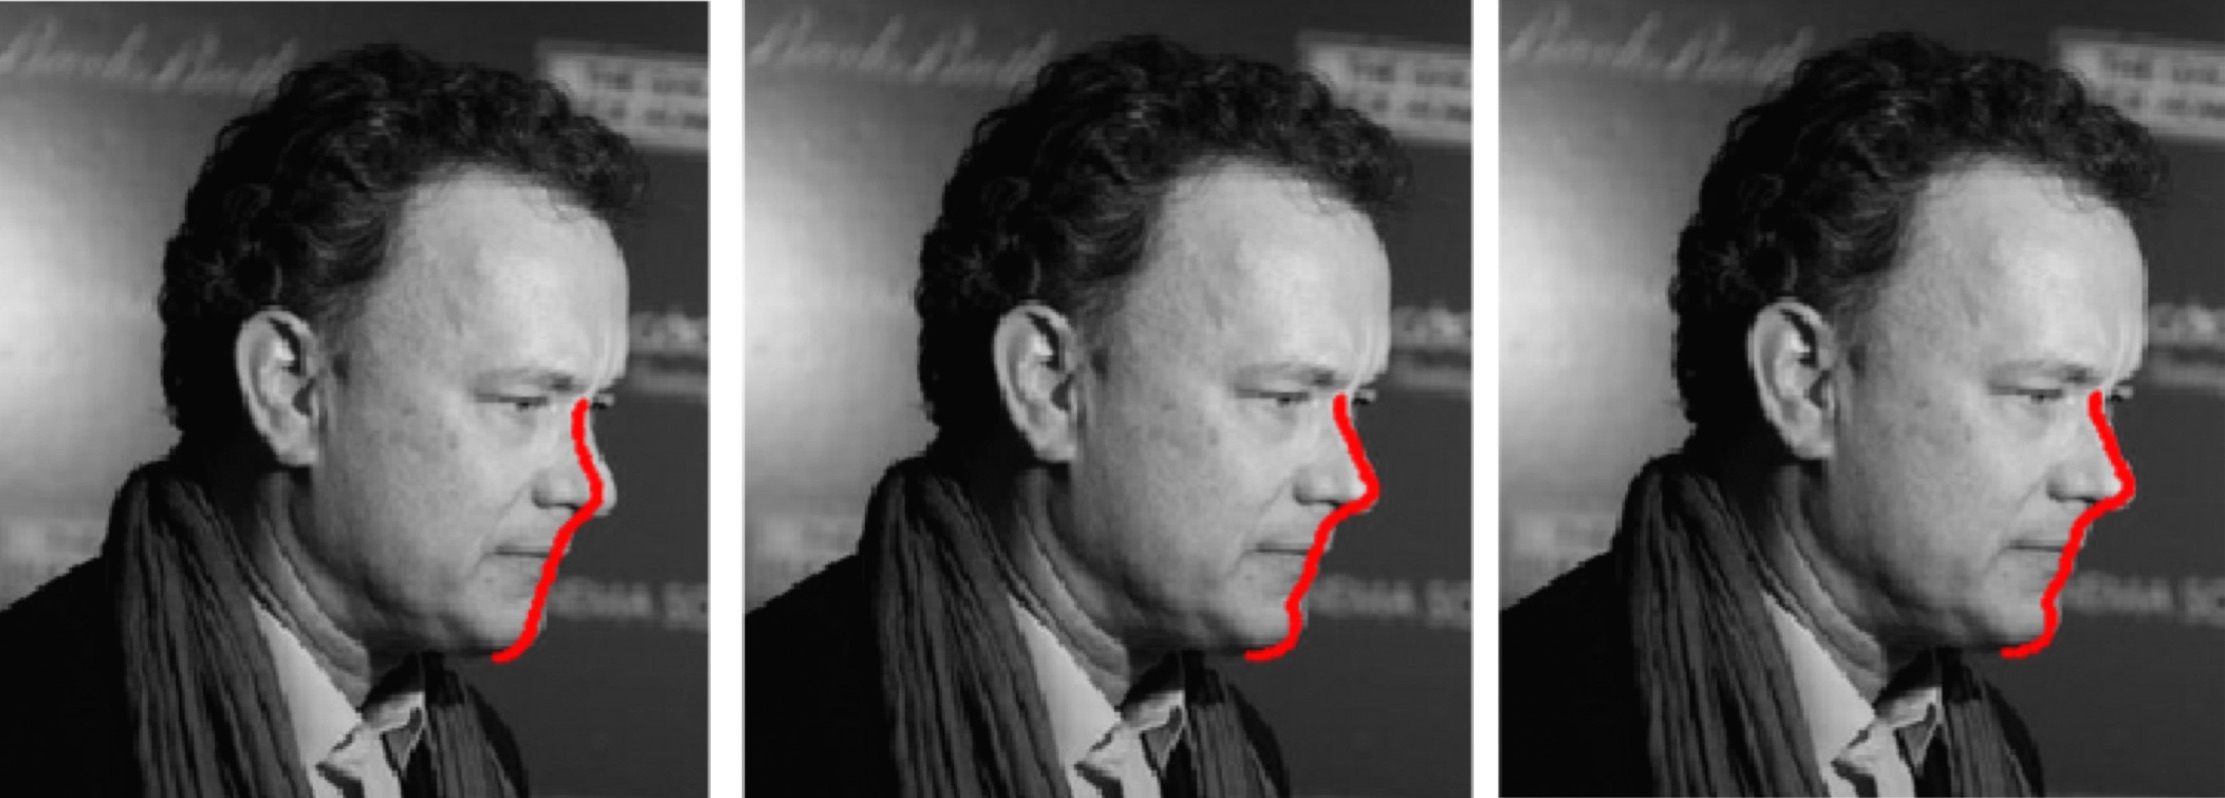
\includegraphics[width=1\linewidth]{figures/ite_th.jpg}
  % replacing the above command with the one below will explicitly set
  % the bounding box of the PS figure to the rectangle (xl,yl),(xh,yh).
  % It will also prevent LaTeX from reading the PS file to determine
  % the bounding box (i.e., it will speed up the compilation process)
  % 
\includegraphics[width=1.5\linewidth, bb=39 696 126 756]{sampleFig}
  %
  %\parbox[t]{.9\columnwidth}{\relax
   %        For all figures please keep in mind that you \textbf{must not}
    %       use images with transparent background! 
     %      }
  %
  \caption{\label{fig:firstExample}
           The silhouette on the 3D mesh projected to the image (red points) in iteration 1, 4 and 7 of our main iteration loop (Section~\ref{sec:silhouetteconstraints}). The silhouette gets closer and closer to the real silhouette as the iteration progresses. We update the silhouette points on the 3D mesh in each iteration.}
\end{figure}

\begin{figure}[t]
  \centering
  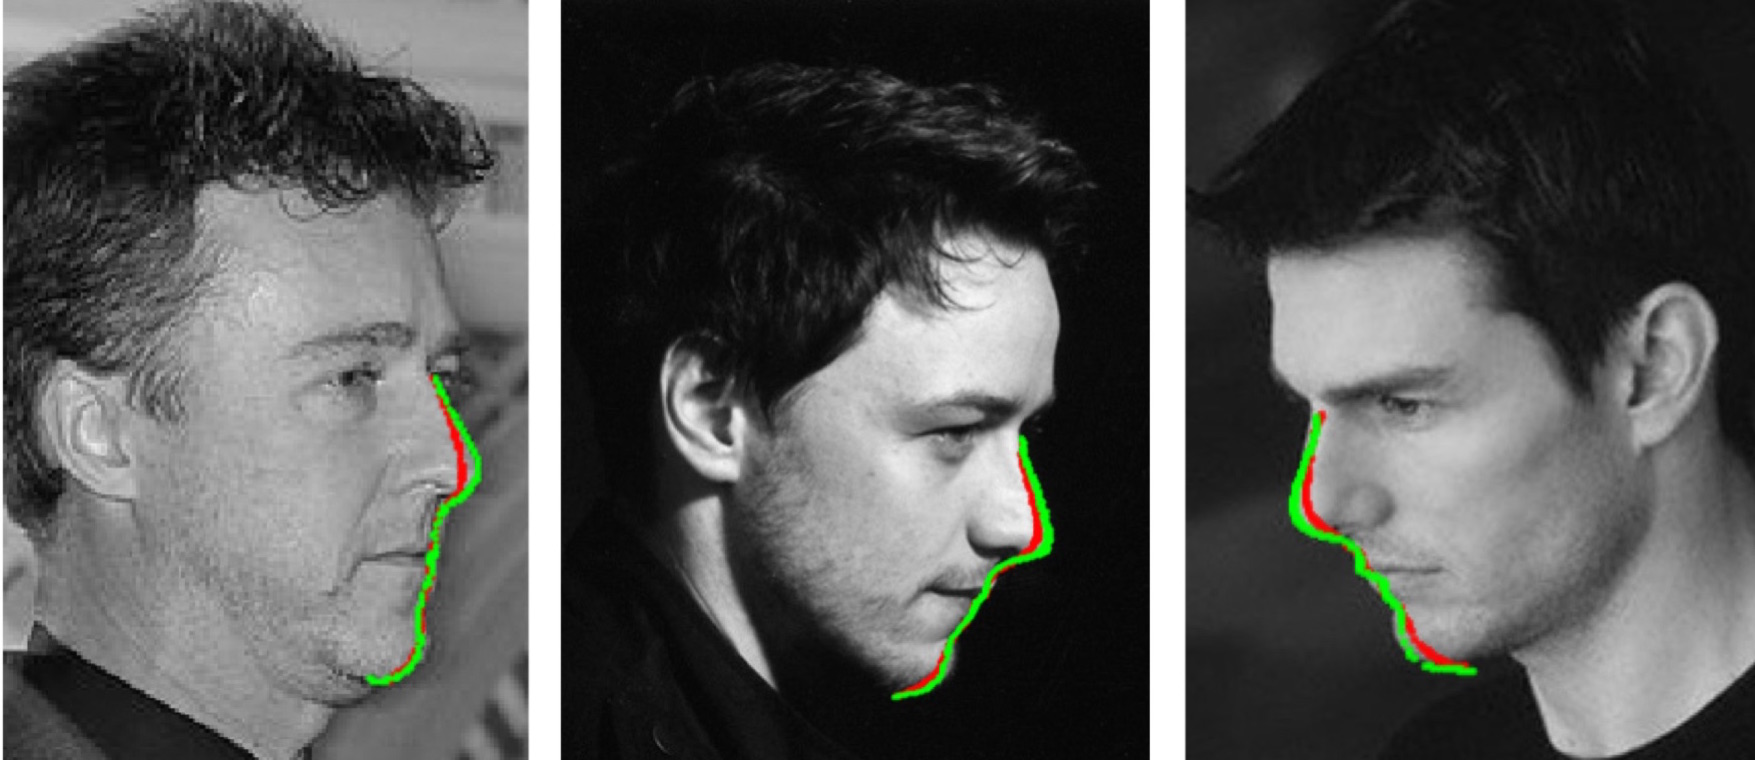
\includegraphics[width=1\linewidth]{figures/sil_all3.jpg}
  % \includegraphics[width=1.5\linewidth]{sil}
  %
  %\parbox[t]{.9\columnwidth}{\relax
   %        For all figures please keep in mind that you \textbf{must not}
    %       use images with transparent background! 
     %      }
  %
  \caption{\label{fig:sil_all}
           We compare 3D silhouette points projected onto input images that were obtained after convergence with our silhouette constraints (green points) and without (red points) for three different individuals. Our approach clearly leads to a more faithful reconstruction of the true silhouettes in the input images.}
\end{figure}

\textbf{Ground-truth Comparison.} Figure~\ref{fig:groundtruth} shows a comparison of our approach with silhouette constraints to the technique by Roth et al. \cite{Roth:2015:UFR} with respect to a ground truth 3D geometry obtained using an Artec Eva 3D scanner. We use 807 images of the volunteer. We align the reconstructed faces with the ground truth using the landmarks on the two meshes. Then, we compute the Euclidean distance from each vertex on the ground truth to the closest point on the reconstructed mesh and normalize the distances. Figure~\ref{fig:groundtruth} shows a color coded visualization of the distances, where red corresponds to big distances to the ground truth, and green represents small distances. We observe that our result matches better the ground truth especially in the area around the nose and the chin. 

\begin{figure}[htb]

   \includegraphics[height=.4\linewidth,width=.3\linewidth,trim=130  -40 100 0,clip]{figures/groundtruth/roth_attila_front2.eps}  
  \includegraphics[height=.41\linewidth,width=.3\linewidth,trim=130  -40 100 0,clip]{figures/groundtruth/attila_front.eps}  
  \includegraphics[height=.41\linewidth,width=.3\linewidth,trim=120  -40 100 -0,clip]{figures/groundtruth/exp_gt_front.eps}    
  
  \includegraphics[height=.41\linewidth,width=.3\linewidth,trim=130  -40 120 0,clip]{figures/groundtruth/roth_attila_profile2}  
  \includegraphics[height=.41\linewidth,width=.3\linewidth,trim=130  -40 100 0,clip]{figures/groundtruth/attila_profile.eps}  
  \includegraphics[height=.41\linewidth,width=.3\linewidth,trim=130  -50 100 0,clip]{figures/groundtruth/exp_gt_profile.eps}  
  
   \includegraphics[height=.41\linewidth,width=.3\linewidth,trim=110  -60 80 0,clip]{figures/groundtruth/roth_attila_front.eps}  
  \includegraphics[height=.41\linewidth,width=.3\linewidth,trim=110  -60 80 0,clip]{figures/groundtruth/exp_front.eps}  
  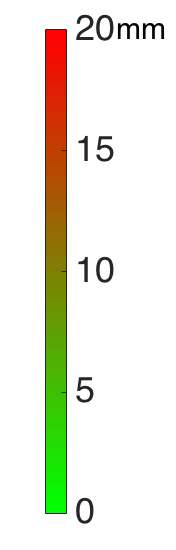
\includegraphics[height=.41\linewidth,width=.3\linewidth,trim=-20  0 -50 0,clip]{figures/groundtruth/colorbar.png} 
   
  \centering
  % the following command controls the width of the embedded PS file
  % (relative to the width of the current column)
 % 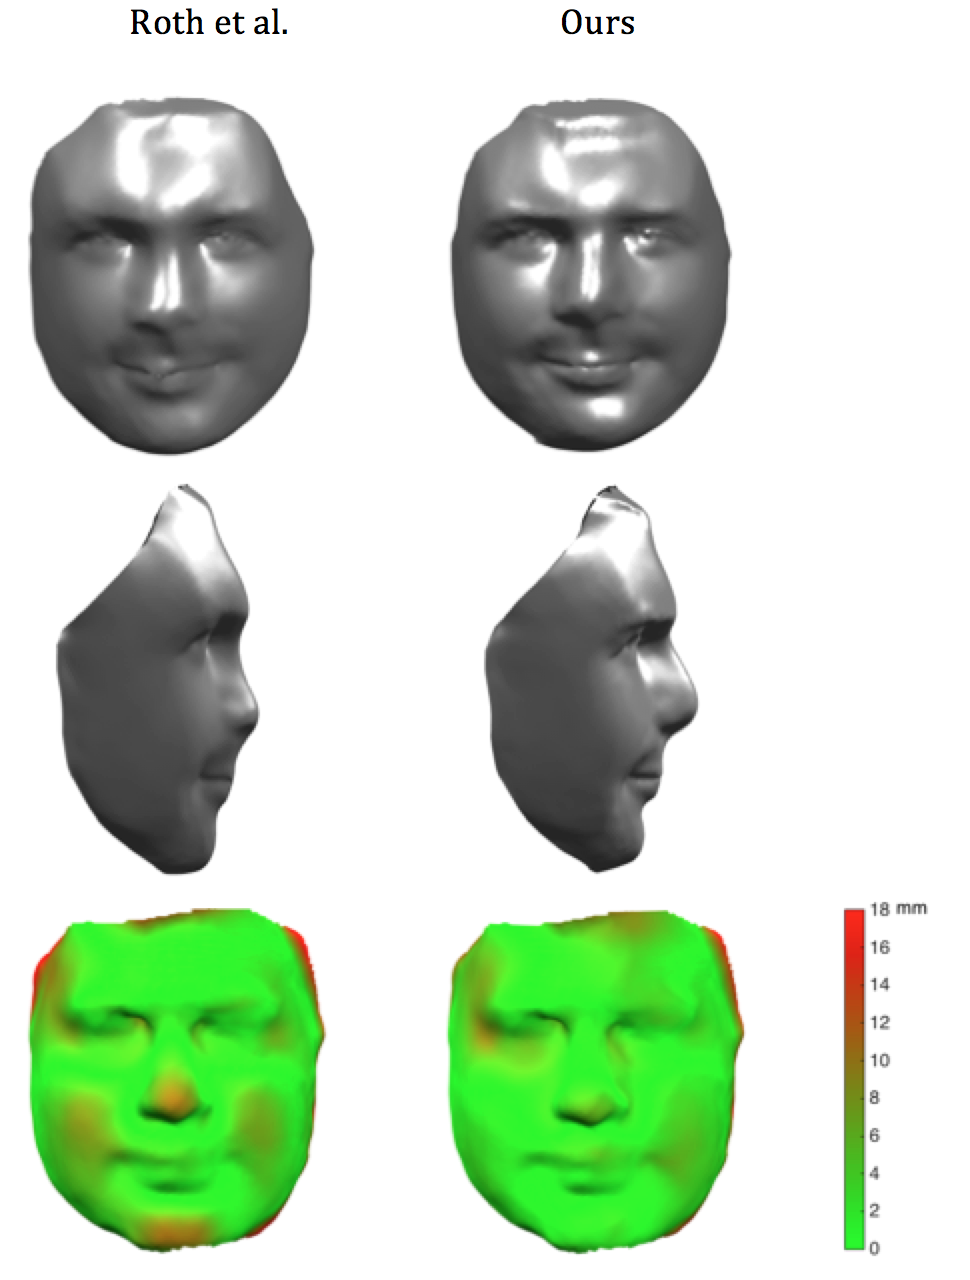
\includegraphics[width=1\linewidth]{figures/ground_truth3.png}
 
  % replacing the above command with the one below will explicitly set
  % the bounding box of the PS figure to the rectangle (xl,yl),(xh,yh).
  % It will also prevent LaTeX from reading the PS file to determine
  % the bounding box (i.e., it will speed up the compilation process)
  % 
\includegraphics[width=1.5\linewidth, bb=39 696 126 756]{sampleFig}
  %
  %\parbox[t]{.9\columnwidth}{\relax
   %        For all figures please keep in mind that you \textbf{must not}
    %       use images with transparent background! 
     %      }
  %
  \caption{\label{fig:groundtruth}
           Distance visualization between a ground truth 3D face acquired using an Artec Eva 3D scanner, and reconstructed faces without (left) and with (right) the silhouette constraints. Red indicates larger distances and green smaller ones. Using silhouette constraints leads to smaller errors in particular in the area around the nose. The range of the distance is 0-20mm from green to red. The 1st column are the results from ~\cite{Roth:2015:UFR}, the 2nd column are our results. }
\end{figure}

%From the result in Figure~\ref{fig:all} we can see, compared with the previous method, our result has obvious improvement on the nose and the chin, as well as the eyes. In each iteration, the mesh is closer and closer to the real geometry, then the 3D face has better correspondence to images. A good correspondence is vital to create the reflectance intensity matrix $M$. The normals to reconstruct face is mainly from photometric stereo approach. Except the nose and chin, the silhouette constraint can improve the whole face quality.

We plot the results in Figure~\ref{fig:all}. To compare the results , we re-implement the method in ~\cite{Roth:2015:UFR}. We test their method with the same dataset used in our implementation. We also generated results with the code made available by Roth et al. ~\cite{Roth:2015:UFR}, but unfortunately this produced inferior results as shown in Figure~\ref{fig:all_roth} . Since they only provide a binary executable, we could not investigate the cause of this issue further.
%-------------------------------------------------------------------------
\section{Conclusions}
\label{sec:conclusions}

We described a method for unconstrained 3D face reconstruction for image collections of individuals dowloaded from the internet, which exhibit unknown illumination, pose, and facial expressions. Our key idea is to introduce silhouette constraints, which are iteratively extracted and updated on the reconstructed 3D mesh, and put into correspondence with edges in each input image. We demonstrate that taking into account our silhouette constraints generally leads to more detailed and accurate 3D reconstructions. In the future, we believe that unconstrained face recognition can be further improved by using dynamic expression models, instead of a single template mesh with a neutral facial expression.


%--------------------------------------------------------------------------
\section{Acknowledgement}
\label{sec:acknowledgement}

This work was supported by Swiss National Science Foundation 200021$\_$156253.

%-------------------------------------------------------------------------


%-------------------------------------------------------------------------
\newpage

%\bibliographystyle{eg-alpha}
\bibliographystyle{eg-alpha-doi}

\bibliography{egbibsample}

\begin{figure*}[tbp]
  \centering
  %\mbox{} \hfill

 % 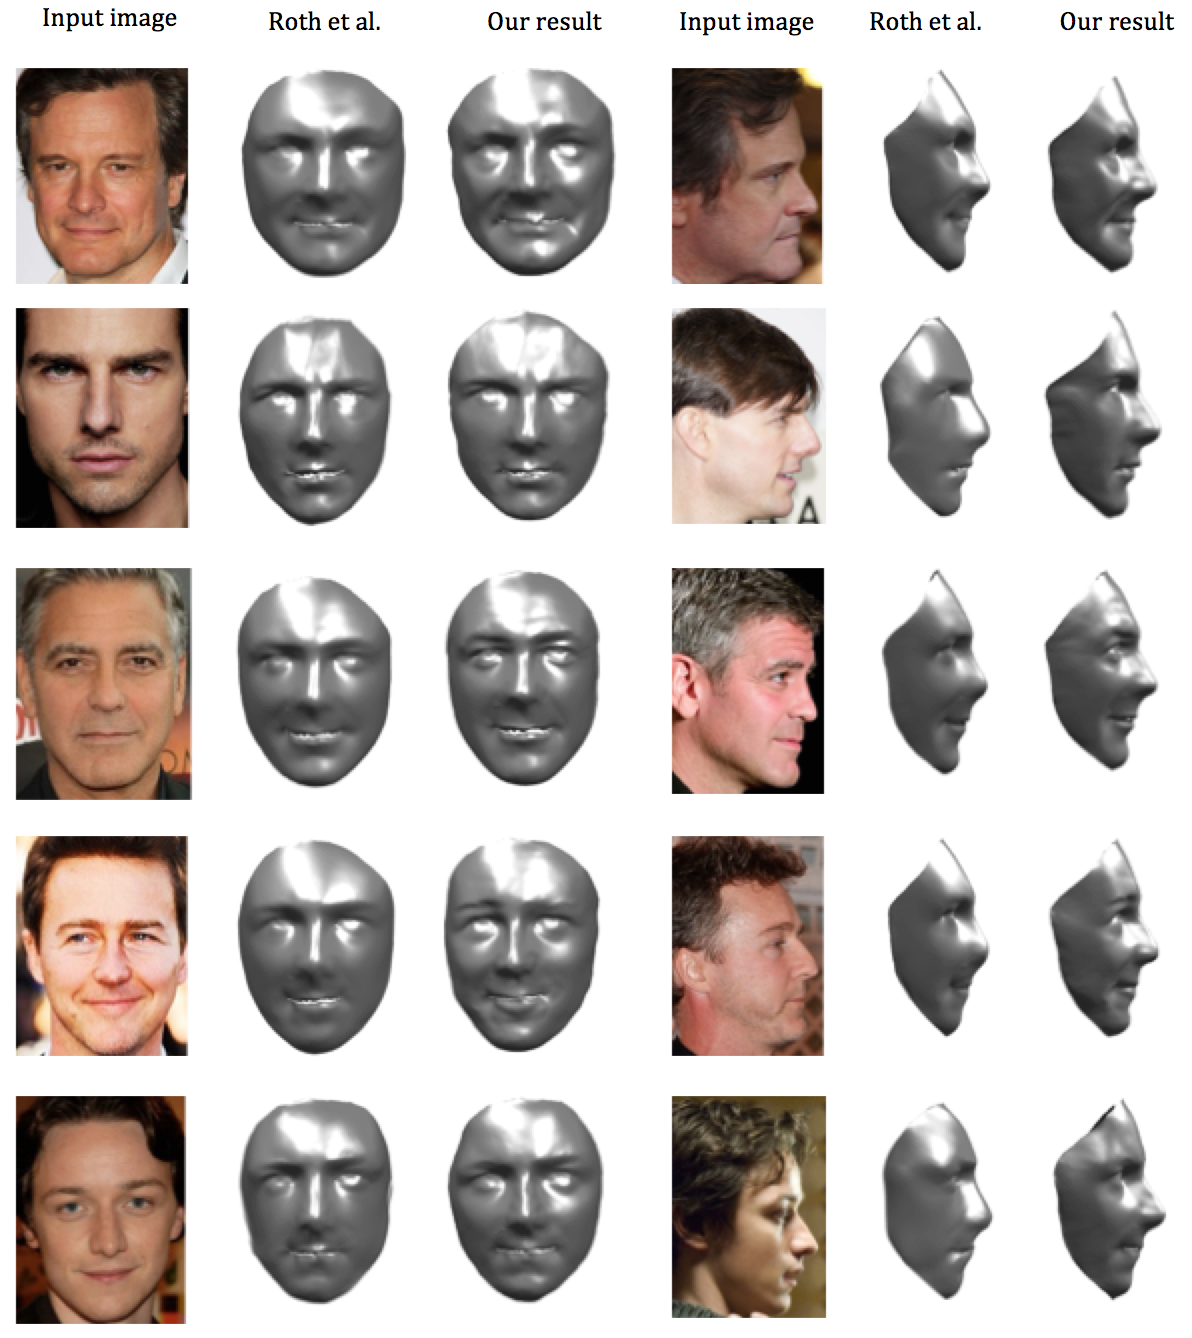
\includegraphics[width=.9\linewidth]{figures/all.png}
  % replacing the above command with the one below will explicitly set
  % the bounding box of the PS figure to the rectangle (xl,yl),(xh,yh).
  % It will also prevent LaTeX from reading the PS file to determine
  % the bounding box (i.e., it will speed up the compilation process)
  % 
\includegraphics[width=.3\linewidth, bb=39 696 126 756]{sampleFig}
  
 
 
   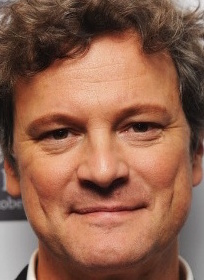
\includegraphics[height=.21\linewidth,width=.15\linewidth,trim=0  -20 0 0]{figures/exp/cf_front.jpg}  
  \includegraphics[height=.21\linewidth,width=.15\linewidth,trim=130  -40 100 0,clip]{figures/exp/roth_cf_front.eps}  
  \includegraphics[height=.21\linewidth,width=.15\linewidth,trim=130  -40 100 0,clip]{figures/exp/cf_front.eps}    
  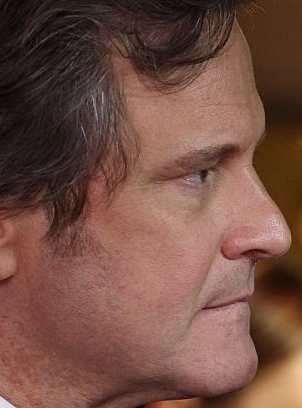
\includegraphics[height=.21\linewidth,width=.15\linewidth,trim=0  -20 0 0]{figures/exp/cf_profile.jpg}
  \includegraphics[height=.21\linewidth,width=.15\linewidth,trim=130  -40 110 -10,clip]{figures/exp/roth_cf_profile.eps}  
   \includegraphics[height=.21\linewidth,width=.15\linewidth,trim=130  -40 90 0,clip]{figures/exp/cf_profile.eps}  
   
      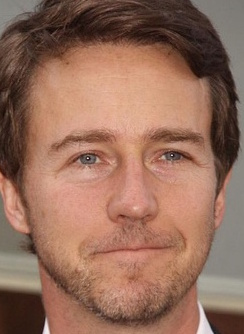
\includegraphics[height=.21\linewidth,width=.15\linewidth,,trim=0  -20 0 0]{figures/exp/ed_front.jpg}  
  \includegraphics[height=.21\linewidth,width=.15\linewidth,,trim=130  -40 90 -10,clip]{figures/exp/roth_ed_front.eps}  
  \includegraphics[height=.21\linewidth,width=.15\linewidth,trim=130  -40 90 0,clip]{figures/exp/ed_front.eps}    
  
\includegraphics[height=.21\linewidth,width=.15\linewidth,,trim=0  -20 0 0]{figures/exp/ed_profile.jpg}
  \includegraphics[height=.21\linewidth,width=.15\linewidth,trim=130  -40 110 -10,clip]{figures/exp/roth_ed_profile.eps}  
   \includegraphics[height=.21\linewidth,width=.15\linewidth,trim=130  -40 90 0,clip]{figures/exp/ed_profile.eps}  
   
         
\includegraphics[height=.21\linewidth,width=.15\linewidth,,trim=0  -20 0 0]{figures/exp/gc_front.jpg}  
  \includegraphics[height=.21\linewidth,width=.15\linewidth,trim=130  -40 90 0,clip]{figures/exp/roth_gc_front.eps}  
  \includegraphics[height=.21\linewidth,width=.15\linewidth,trim=130  -40 90 0,clip]{figures/exp/gc_front.eps}    
  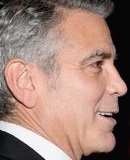
\includegraphics[height=.21\linewidth,width=.15\linewidth,,trim=0  -20 0 0]{figures/exp/gc_profile.jpg}
  \includegraphics[height=.21\linewidth,width=.15\linewidth,trim=130  -40 110 0,clip]{figures/exp/roth_gc_profile.eps}  
   \includegraphics[height=.21\linewidth,width=.15\linewidth,trim=130  -40 100 0,clip]{figures/exp/gc_profile.eps}  
   
   
         
\includegraphics[height=.21\linewidth,width=.15\linewidth,,trim=0  -10 0 0]{figures/exp/tc_front.jpg}  
  \includegraphics[height=.21\linewidth,width=.15\linewidth,trim=130  -40 90 -10,clip]{figures/exp/roth_tc_front.eps}  
  \includegraphics[height=.21\linewidth,width=.15\linewidth,trim=130  -40 90 0,clip]{figures/exp/tc_front.eps}    
  
\includegraphics[height=.21\linewidth,width=.15\linewidth,,trim=0  -20 0 0]{figures/exp/tc_profile.jpg}
  \includegraphics[height=.21\linewidth,width=.15\linewidth,trim=130  -40 100 0,clip]{figures/exp/roth_tc_profile.eps}  
   \includegraphics[height=.21\linewidth,width=.15\linewidth,trim=130  -40 100 0,clip]{figures/exp/tc_profile.eps}  
   
   
\includegraphics[height=.21\linewidth,width=.15\linewidth,,trim=0  -20 0 0]{figures/exp/wm_front.jpg}  
  \includegraphics[height=.21\linewidth,width=.15\linewidth,trim=130  -40 90 0,clip]{figures/exp/roth_wm_front.eps}  
  \includegraphics[height=.21\linewidth,width=.15\linewidth,trim=130  -40 90 0,clip]{figures/exp/wm_front.eps}    
  \includegraphics[height=.21\linewidth,width=.15\linewidth,trim=0  -20 0 0]{figures/exp/wm_profile.jpg}
  \includegraphics[height=.20\linewidth,width=.15\linewidth,trim=130  -40 110 0,clip]{figures/exp/roth_wm_profile.eps}  
   \includegraphics[height=.21\linewidth,trim=130  -40 90 0,clip]{figures/exp/wm_profile.eps}  
    
  \caption{\label{fig:all}%
           Comparison results of different individuals between the state of the art technique by Roth et al.~\cite{Roth:2015:UFR} and our approach. The 2nd and 5th column are the results from ~\cite{Roth:2015:UFR}, the 3rd and 6th column are our results.  In our results, the nose and chin areas generally fit better to the real image. Our results tend to exhibit less oversmoothing and more geometric detail also around the eyes.
           \newline
  }
\end{figure*}

\begin{figure*}[tbp]
  \centering
  %\mbox{} \hfill
  
   \includegraphics[height=.21\linewidth, width=.15\linewidth,trim=0  -20 0 0]{figures/teaser/bw_front.jpg}  
  \includegraphics[height=.21\linewidth,width=.16\linewidth,trim=0  -20 0 0]{figures/teaser/bw_roth_front.png}  
  \includegraphics[height=.21\linewidth,width=.16\linewidth,trim=130  -40 90 0,clip]{figures/teaser/roth_bw_front.eps}    
  \includegraphics[height=.21\linewidth,width=.15\linewidth,trim=0  -20 0 0]{figures/teaser/bw_profile.jpg}
  \includegraphics[height=.21\linewidth,width=.15\linewidth,trim=0  -20 0 0]{figures/teaser/bw_roth_profile.png}  
  \includegraphics[height=.21\linewidth,trim=130  -40 100 0,clip]{figures/teaser/bw_profile.eps}    
 
   \includegraphics[height=.21\linewidth,width=.15\linewidth,trim=0  -20 0 0]{figures/exp/cf_front.jpg}  
  \includegraphics[height=.21\linewidth,trim=130  -40 100 0,clip]{figures/exp/cf_roth_front.eps}  
  \includegraphics[height=.21\linewidth,width=.15\linewidth,trim=130  -40 100 0,clip]{figures/exp/cf_front.eps}    
  \includegraphics[height=.21\linewidth,width=.15\linewidth,trim=0  -20 0 0]{figures/exp/cf_profile.jpg}
  \includegraphics[height=.21\linewidth,width=.15\linewidth,trim=0  -20 0 0]{figures/exp/cf_roth_profile.png}  
   \includegraphics[height=.21\linewidth,width=.15\linewidth,trim=130  -40 90 0,clip]{figures/exp/cf_profile.eps}  
   
      \includegraphics[height=.21\linewidth,width=.15\linewidth,,trim=0  -20 0 0]{figures/exp/ed_front.jpg}  
  \includegraphics[height=.21\linewidth,width=.15\linewidth,,trim=130  -40 90 -10,clip]{figures/exp/ed_roth_front.eps}  
  \includegraphics[height=.21\linewidth,width=.15\linewidth,trim=130  -40 90 0,clip]{figures/exp/ed_front.eps}    
  \includegraphics[height=.21\linewidth,width=.15\linewidth,,trim=0  -20 0 0]{figures/exp/ed_profile.jpg}
  \includegraphics[height=.21\linewidth,width=.15\linewidth,trim=0  -20 0 0]{figures/exp/ed_roth_profile.png}  
   \includegraphics[height=.21\linewidth,width=.15\linewidth,trim=130  -40 90 0,clip]{figures/exp/ed_profile.eps}  
   
         \includegraphics[height=.21\linewidth,width=.15\linewidth,,trim=0  -20 0 0]{figures/exp/gc_front.jpg}  
  \includegraphics[height=.21\linewidth,width=.15\linewidth,trim=130  -40 90 0,clip]{figures/exp/gc_roth_front.eps}  
  \includegraphics[height=.21\linewidth,width=.15\linewidth,trim=130  -40 90 0,clip]{figures/exp/gc_front.eps}    
  \includegraphics[height=.21\linewidth,width=.15\linewidth,,trim=0  -20 0 0]{figures/exp/gc_profile.jpg}
  \includegraphics[height=.21\linewidth,width=.15\linewidth,,trim=0  -20 0 0]{figures/exp/gc_roth_profile.png}  
   \includegraphics[height=.21\linewidth,width=.15\linewidth,trim=130  -40 90 0,clip]{figures/exp/gc_profile.eps}  
   
   
         \includegraphics[height=.21\linewidth,width=.15\linewidth,,trim=0  -10 0 0]{figures/exp/tc_front.jpg}  
  \includegraphics[height=.21\linewidth,width=.15\linewidth,trim=130  -40 90 -10,clip]{figures/exp/tc_roth_front.eps}  
  \includegraphics[height=.21\linewidth,width=.15\linewidth,trim=130  -40 90 0,clip]{figures/exp/tc_front.eps}    
  \includegraphics[height=.21\linewidth,width=.15\linewidth,,trim=0  -20 0 0]{figures/exp/tc_profile.jpg}
  \includegraphics[height=.21\linewidth,width=.15\linewidth,,trim=0  -20 0 0]{figures/exp/tc_roth_profile.png}  
   \includegraphics[height=.21\linewidth,width=.15\linewidth,trim=130  -40 90 0,clip]{figures/exp/tc_profile.eps}  
   
   \includegraphics[height=.21\linewidth,width=.15\linewidth,,trim=0  -20 0 0]{figures/exp/wm_front.jpg}  
  \includegraphics[height=.21\linewidth,width=.15\linewidth,trim=130  -40 90 0,clip]{figures/exp/wm_roth_front.eps}  
  \includegraphics[height=.21\linewidth,width=.15\linewidth,trim=130  -40 90 0,clip]{figures/exp/wm_front.eps}    
  \includegraphics[height=.21\linewidth,width=.15\linewidth,trim=0  -20 0 0]{figures/exp/wm_profile.jpg}
  \includegraphics[height=.20\linewidth,width=.15\linewidth,,trim=-10  -20 0 0]{figures/exp/wm_roth_profile2.png}  
   \includegraphics[height=.21\linewidth,trim=130  -40 90 0,clip]{figures/exp/wm_profile.eps}  
   

  
  \caption{\label{fig:all_roth}%
           Comparison results of different individuals between the state of the art technique by Roth et al.~\cite{Roth:2015:UFR} and our approach. The 2nd and 5th column are the results from the code made available from ~\cite{Roth:2015:UFR}, the 3rd and 6th column are our results.  
           \newline
  }
\end{figure*}



\end{document}

